%!TEX root = ../thesis.tex

\section{Example executions and worst case scenario}

\subsection{A small example}


\subsection{A example containing a large red face}

Consider the graph given in Figure \ref{fig:ex:vert:graph} this graph has as highest degree vertices two vertices of degree 12. We will show how the proposed algorithm will handle this graph.

The way in which the algorithm handles this graph is far from ideal leading to a 10-sided face. While the provided upperbound would lead to (at worst) a 11-sided \fxnote{11 or 12?} face. Furthermore the approach in this graph is scaleabale as is shown in Figure \ref{some figure TODO Show where to scale using dashed lines etc..}

\begin{figure}[h]
  \centering
  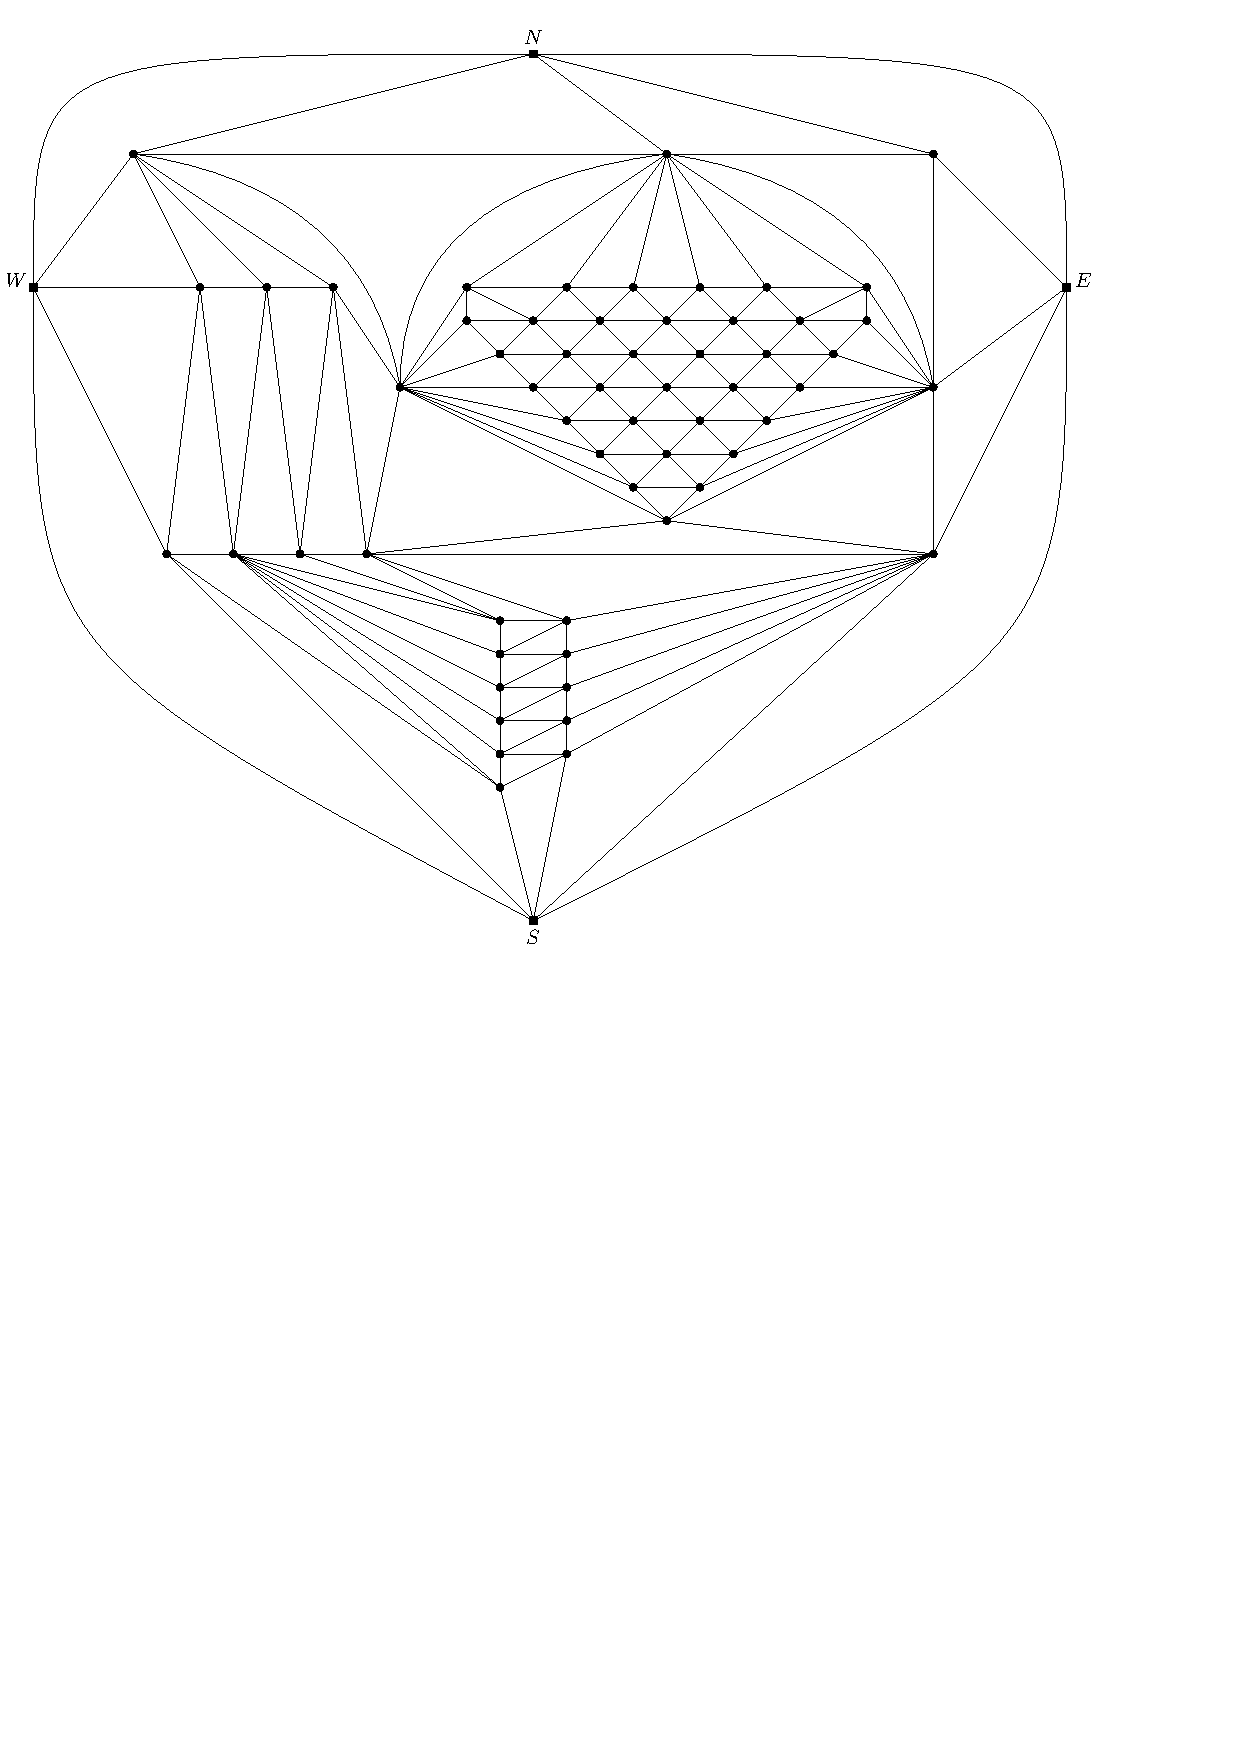
\includegraphics[width=\textwidth]{examples/img/vertWorstCase/graph}
  \caption{}
  \label{fig:ex:vert:graph}
\end{figure}

The application of the algorithm to this graph is quite straightforward. Figures \ref{fig:ex:vert:sweep1} to \ref{fig:ex:vert:sweepfinal} are steps in the sweepline algorithm. This graph does not permit any topfanflips since all large topfans are either incident to a pole or starting above a split vertex. \fxnote{In a sense a pole is a splitvertex}
Then finally the subdivision of large red faces happen in Figures \ref{fig:ex:vert:subdiv1} and \ref{fig:ex:vert:subdivfinal}.

In the captions of the subfigures of Figure \ref{fig:ex:vert} more details about each step can be found.


\begin{figure}
    \centering
    \begin{subfigure}[b]{.9 \textwidth}
      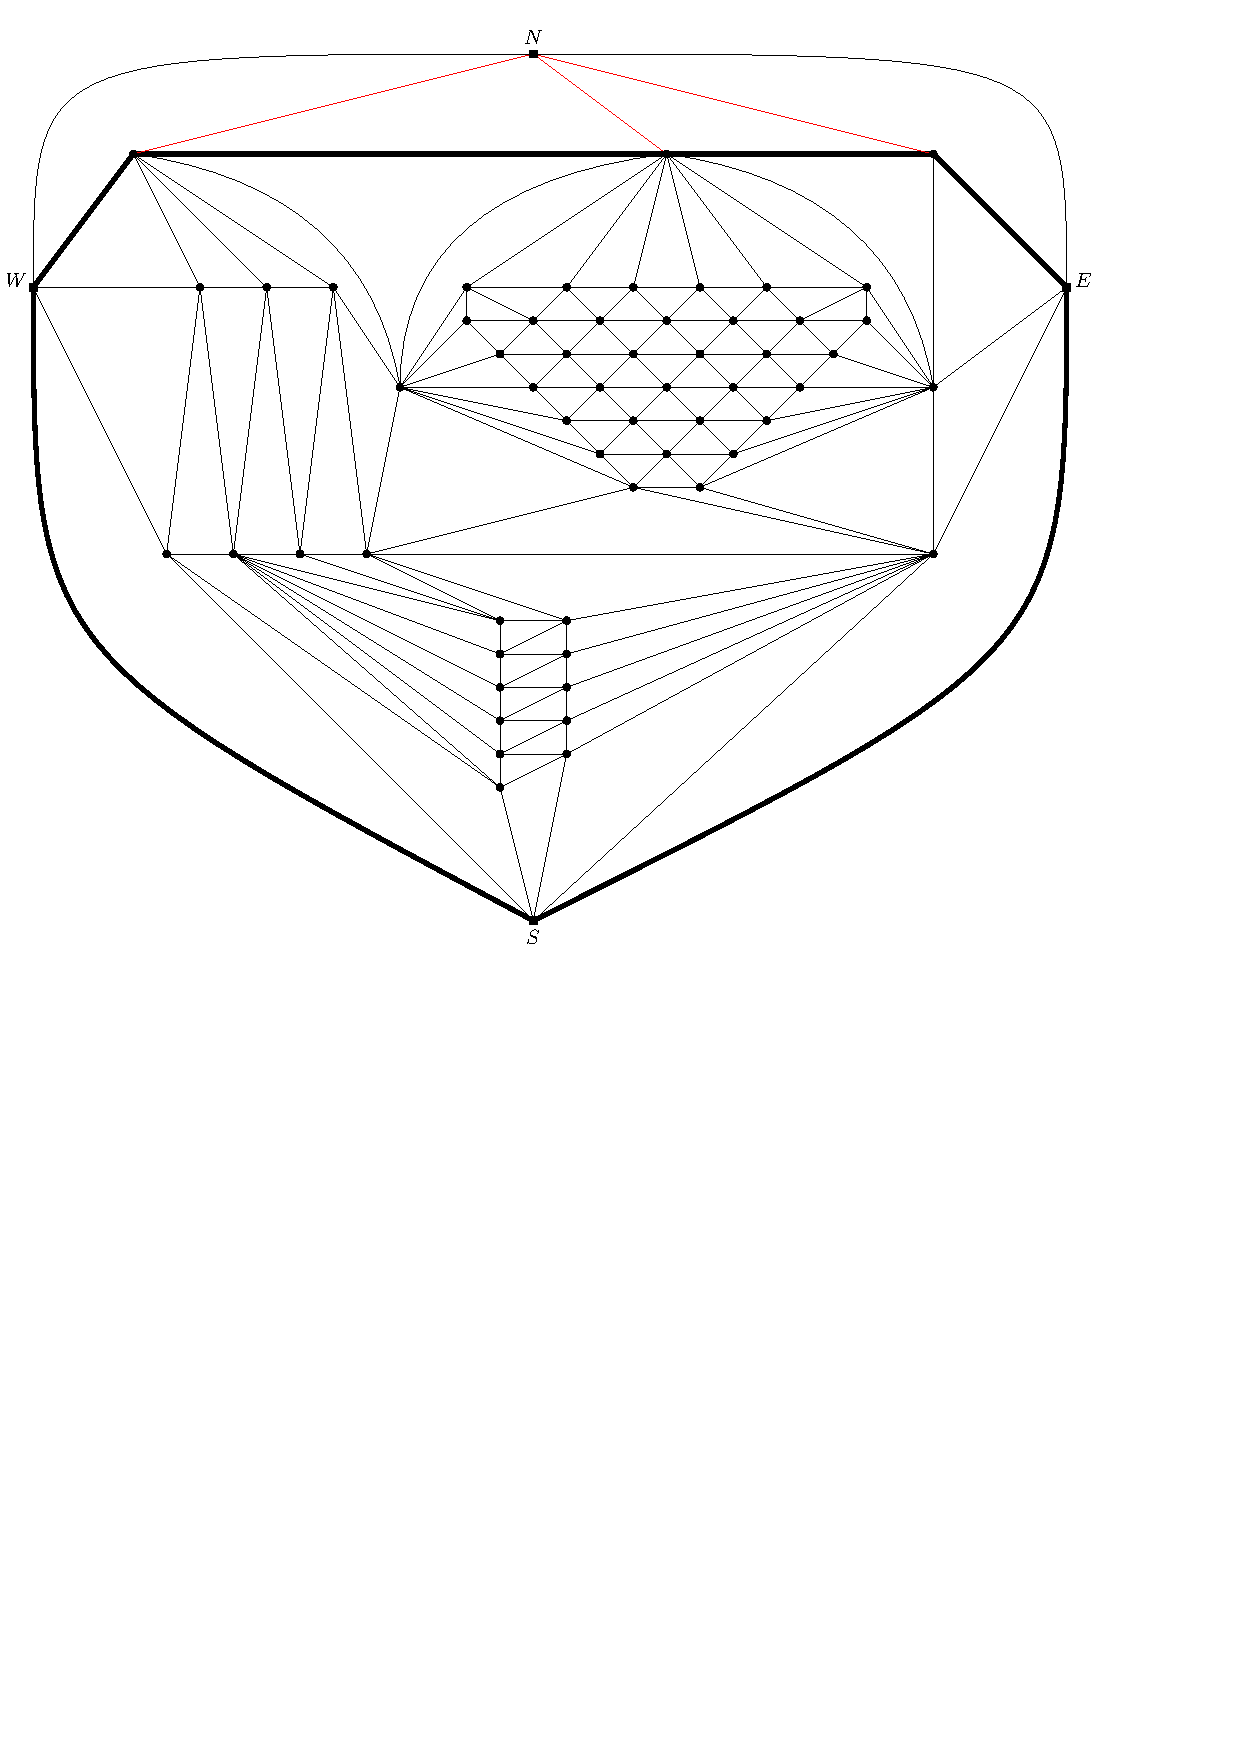
\includegraphics[width=\textwidth]{examples/img/vertWorstCase/sweep1}
      \caption{The initial sweepcycle}
      \label{fig:ex:vert:sweep1}
    \end{subfigure}
    ~
    \begin{subfigure}[b]{.9 \textwidth}
      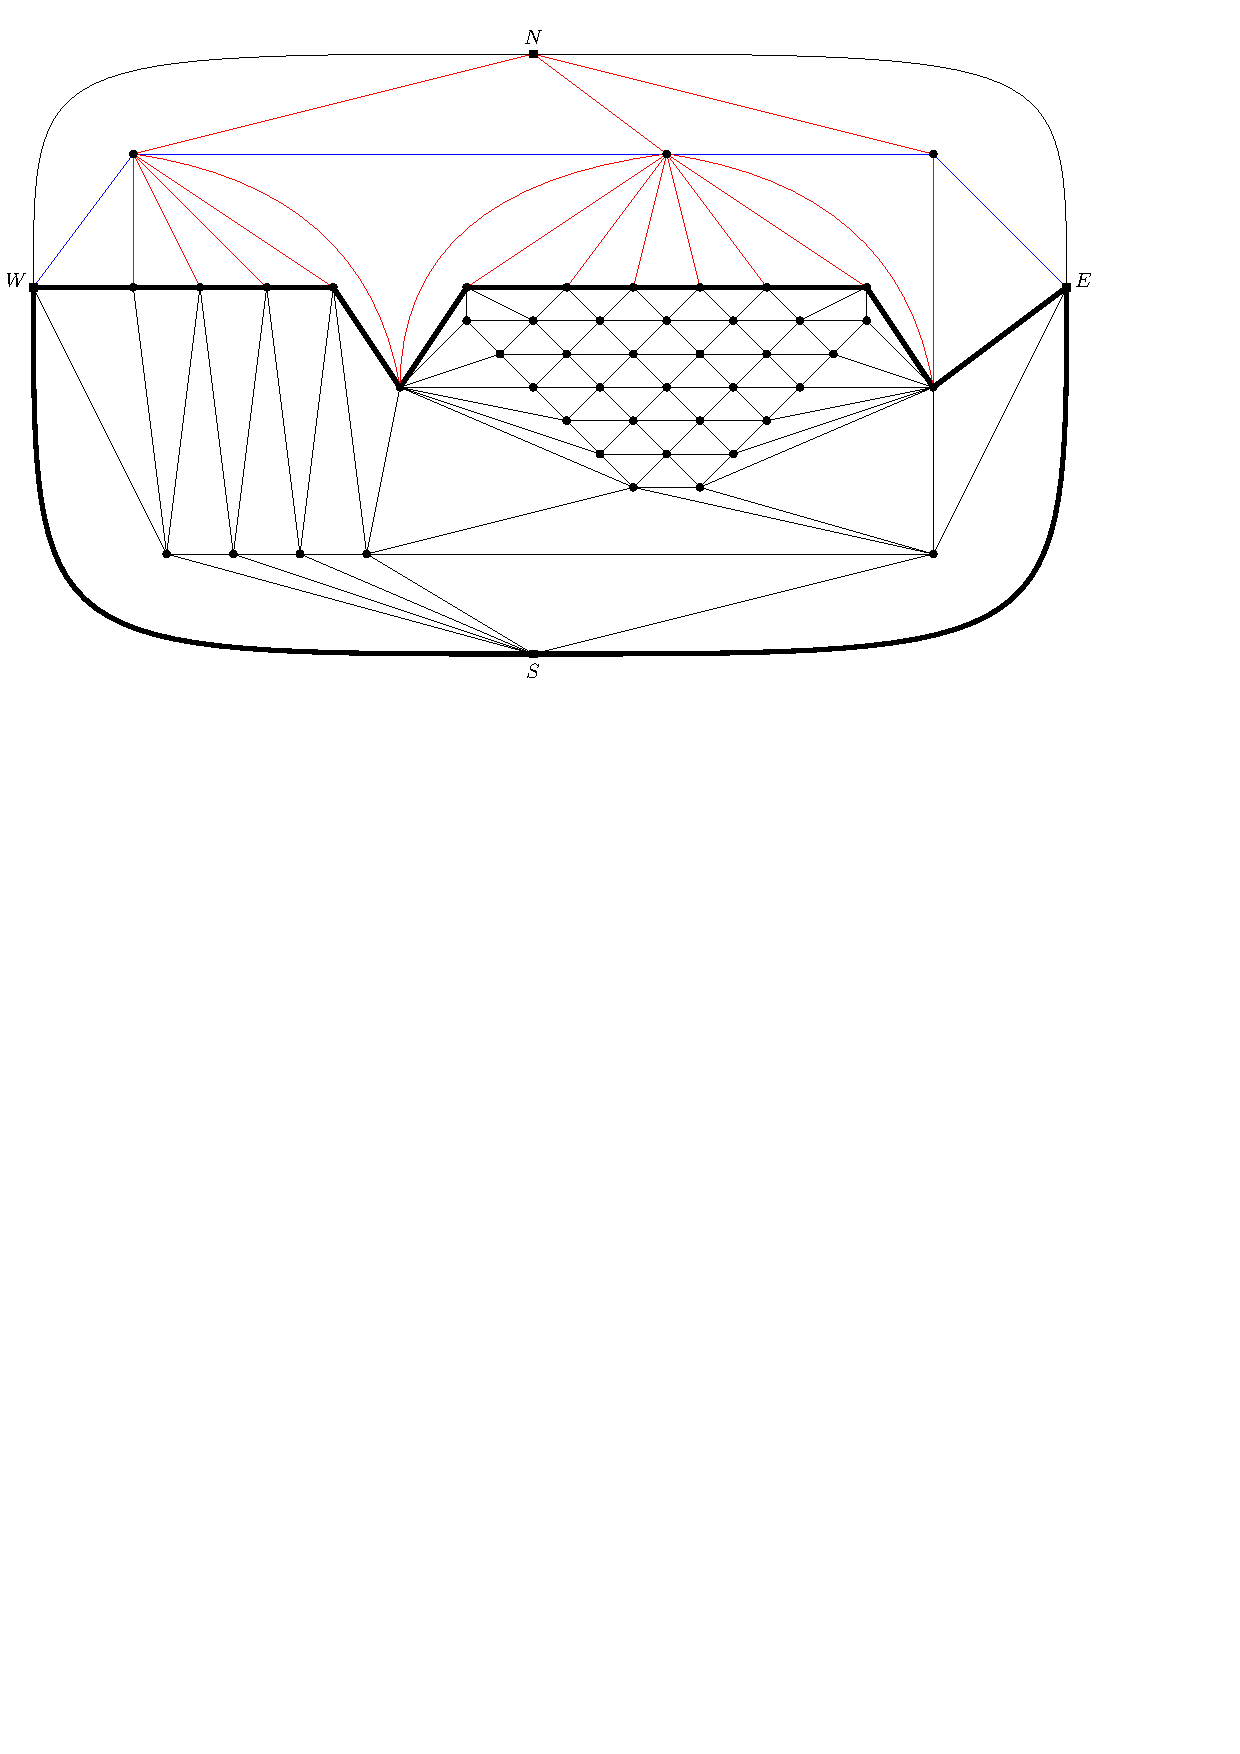
\includegraphics[width=\textwidth]{examples/img/vertWorstCase/sweep2}
      \caption{Advancing by one update of the sweepcycle}
      \label{fig:ex:vert:sweep2}
    \end{subfigure}
    \label{fig:ex:vert}
    \caption{The steps of the algorithm}
\end{figure}

\begin{figure}
    \ContinuedFloat
    \begin{subfigure}[b]{.9 \textwidth}
      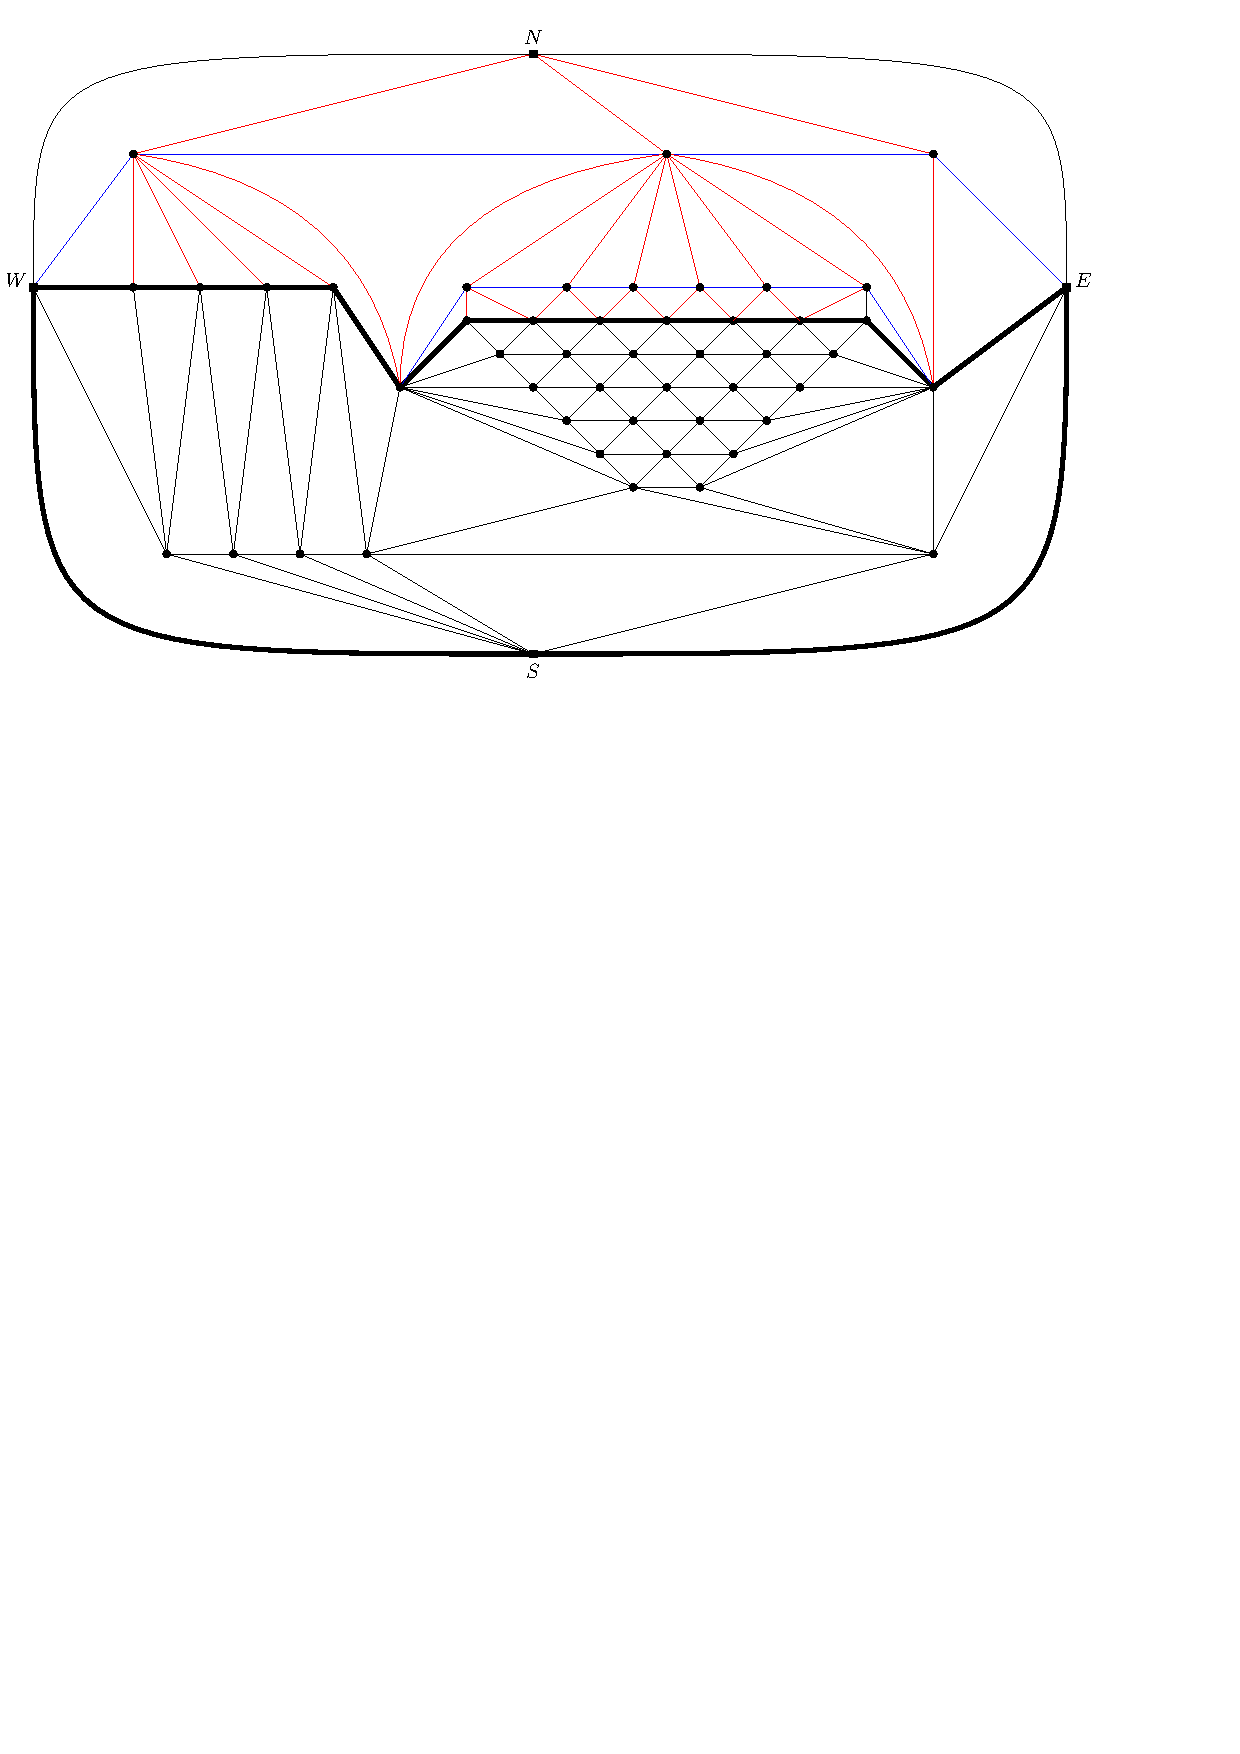
\includegraphics[width=\textwidth]{examples/img/vertWorstCase/sweep3}
      \caption{This update the prefence had a chord leading to this smaller update step}
      \label{fig:ex:vert:sweep3}
    \end{subfigure}
    ~
    \begin{subfigure}[b]{.9 \textwidth}
      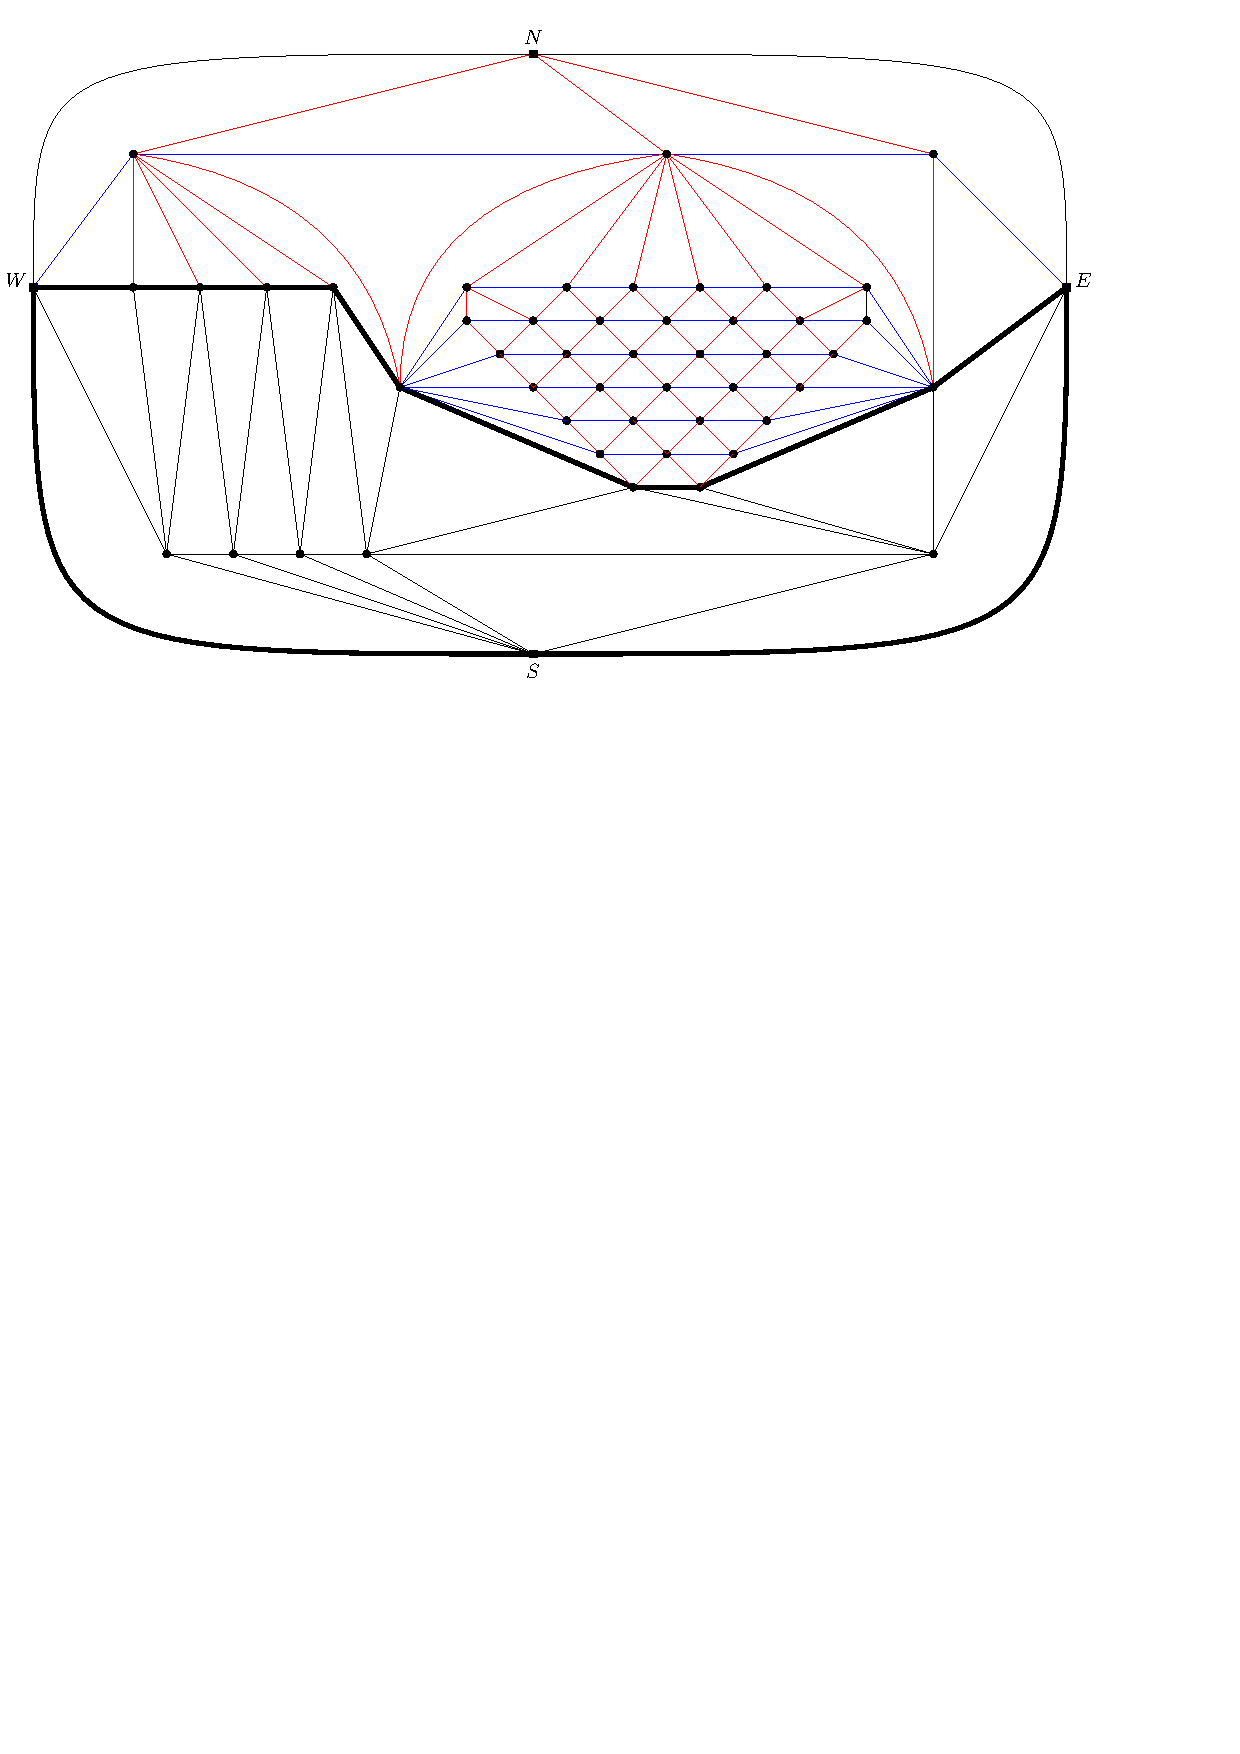
\includegraphics[width=\textwidth]{examples/img/vertWorstCase/sweep4}
      \caption{Several similar update steps combined into one figure}
      \label{fig:ex:vert:sweep4}
    \end{subfigure}
    \caption{The steps of the algorithm}
\end{figure}

\begin{figure}
    \ContinuedFloat
    \begin{subfigure}[b]{.9 \textwidth}
      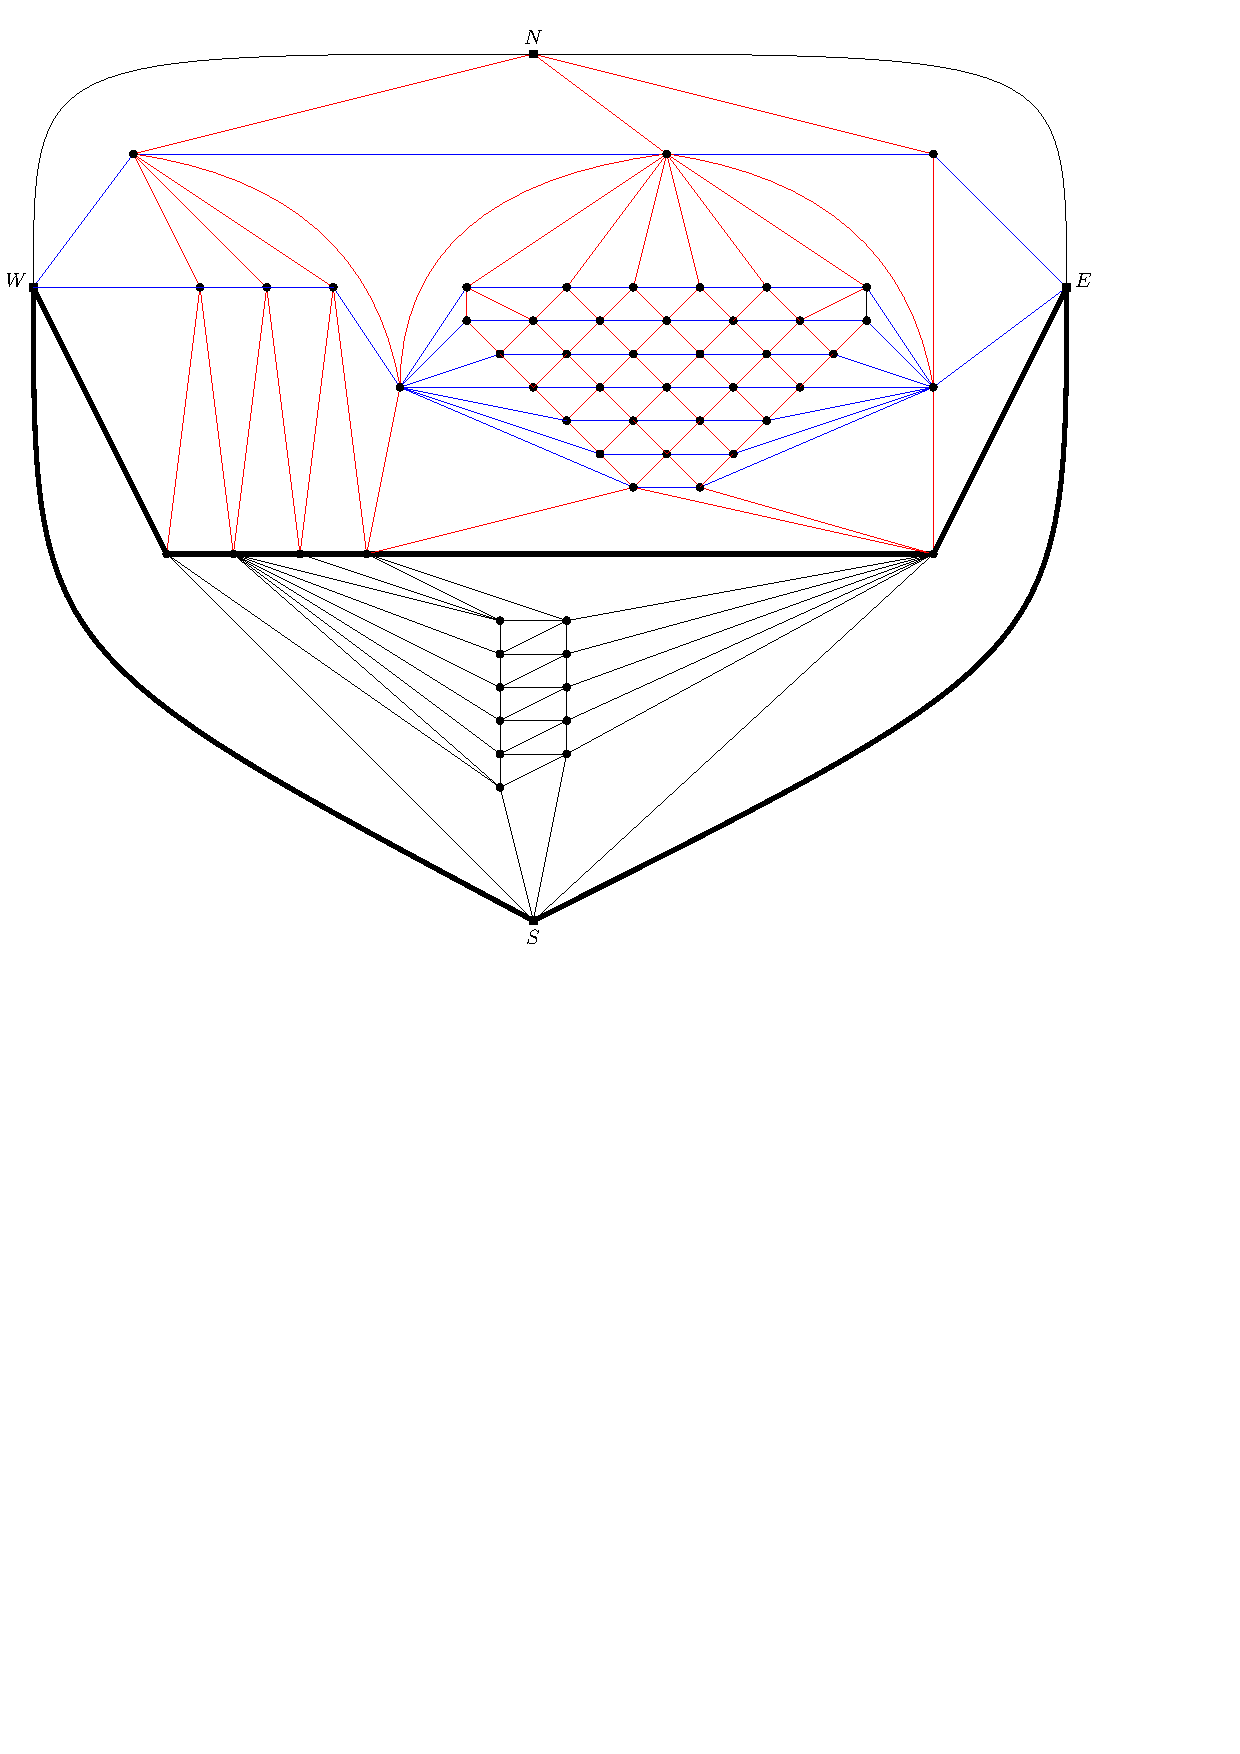
\includegraphics[width=\textwidth]{examples/img/vertWorstCase/sweep5}
      \caption{An update step, this time without irregularities}
      \label{fig:ex:vert:sweep5}
    \end{subfigure}
    ~
    \begin{subfigure}[b]{.9 \textwidth}
      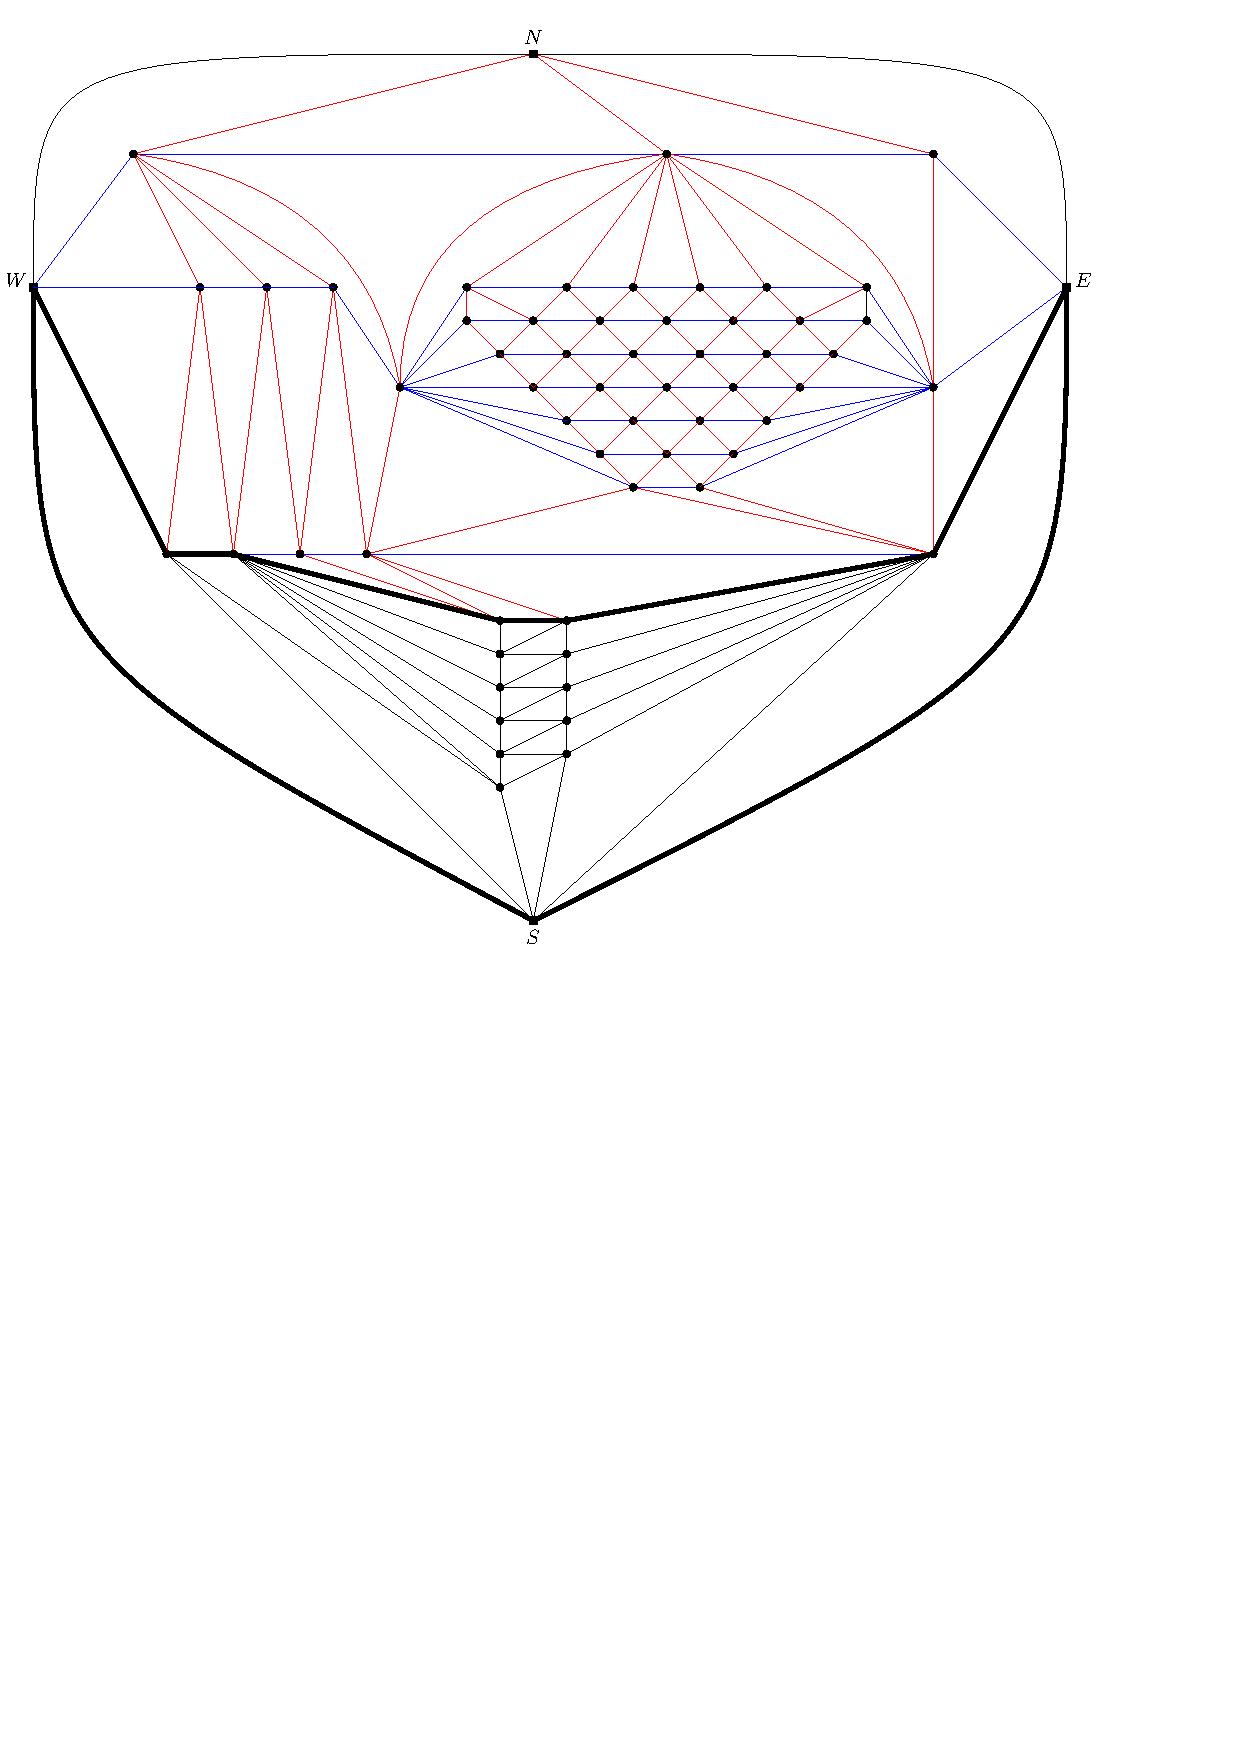
\includegraphics[width=\textwidth]{examples/img/vertWorstCase/sweep6}
      \caption{Another update step. Note that the original prefence would have a polebound 2-chord with the edge $\pE \pS$.}
      \label{fig:ex:vert:sweep6}
    \end{subfigure}
    \caption{The steps of the algorithm}
\end{figure}

\begin{figure}
    \ContinuedFloat
    \begin{subfigure}[b]{.9 \textwidth}
      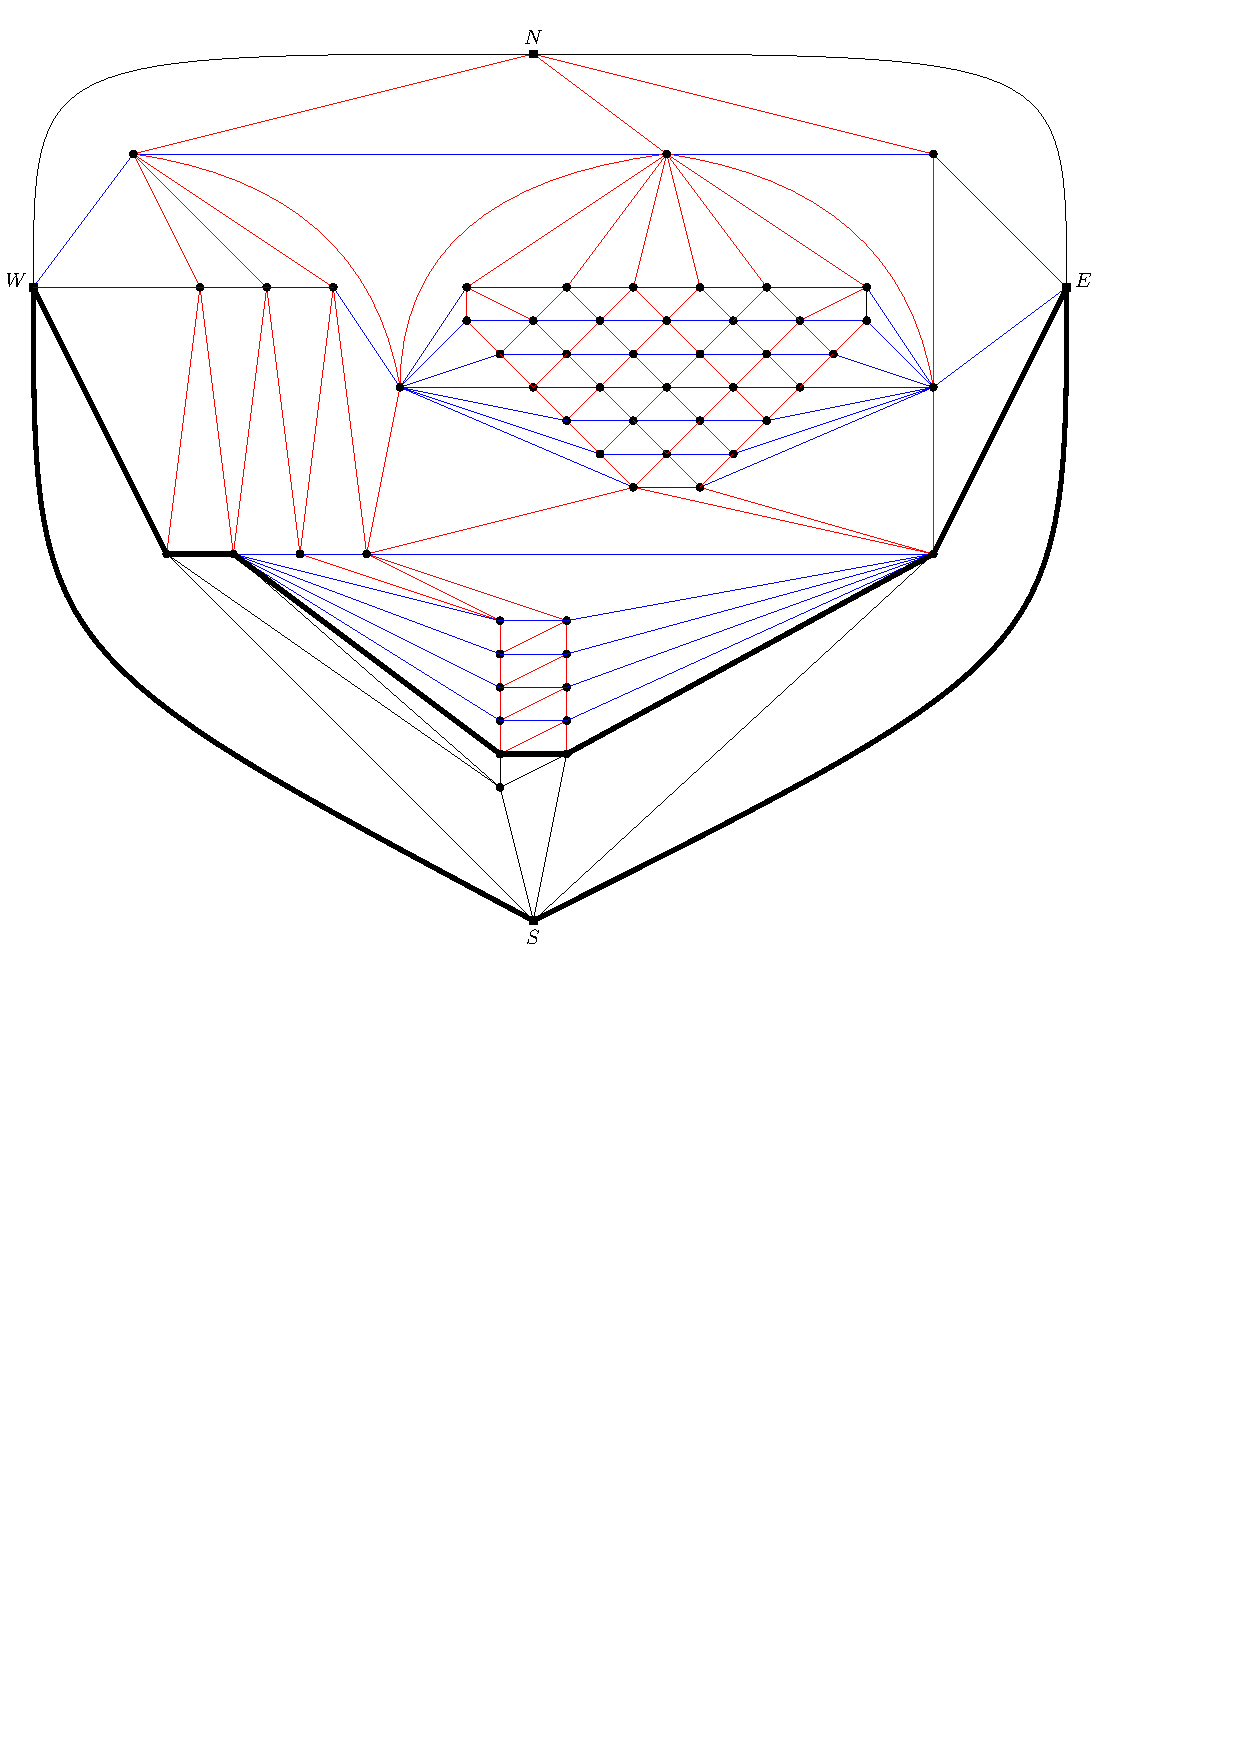
\includegraphics[width=\textwidth]{examples/img/vertWorstCase/sweep7}
      \caption{}
      \label{fig:ex:vert:sweep7}
    \end{subfigure}
    ~
    \begin{subfigure}[b]{.9 \textwidth}
      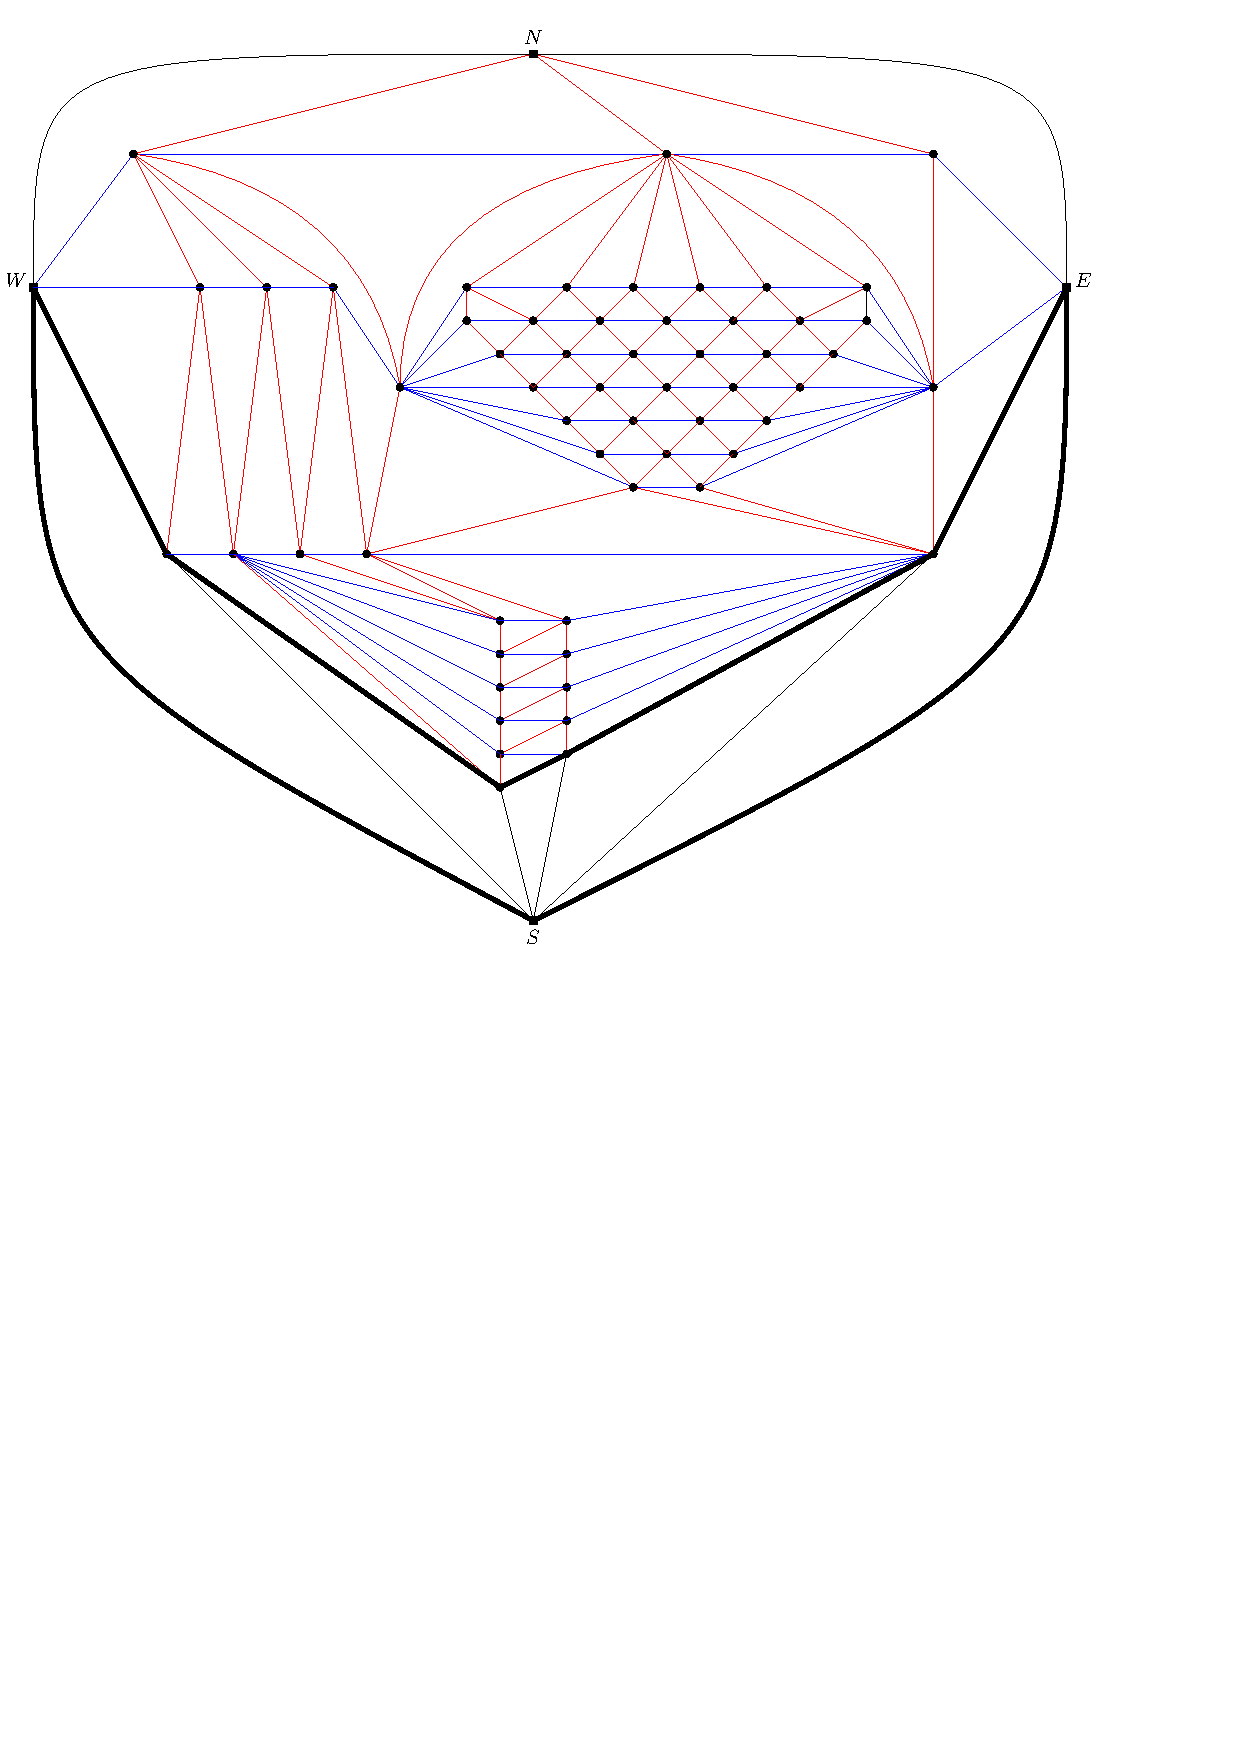
\includegraphics[width=\textwidth]{examples/img/vertWorstCase/sweep8}
      \caption{}
      \label{fig:ex:vert:sweep8}
    \end{subfigure}
  \caption{The steps of the algorithm}
  \label{}

\end{figure}



\begin{figure}
    \ContinuedFloat
    \begin{subfigure}[b]{.9 \textwidth}
      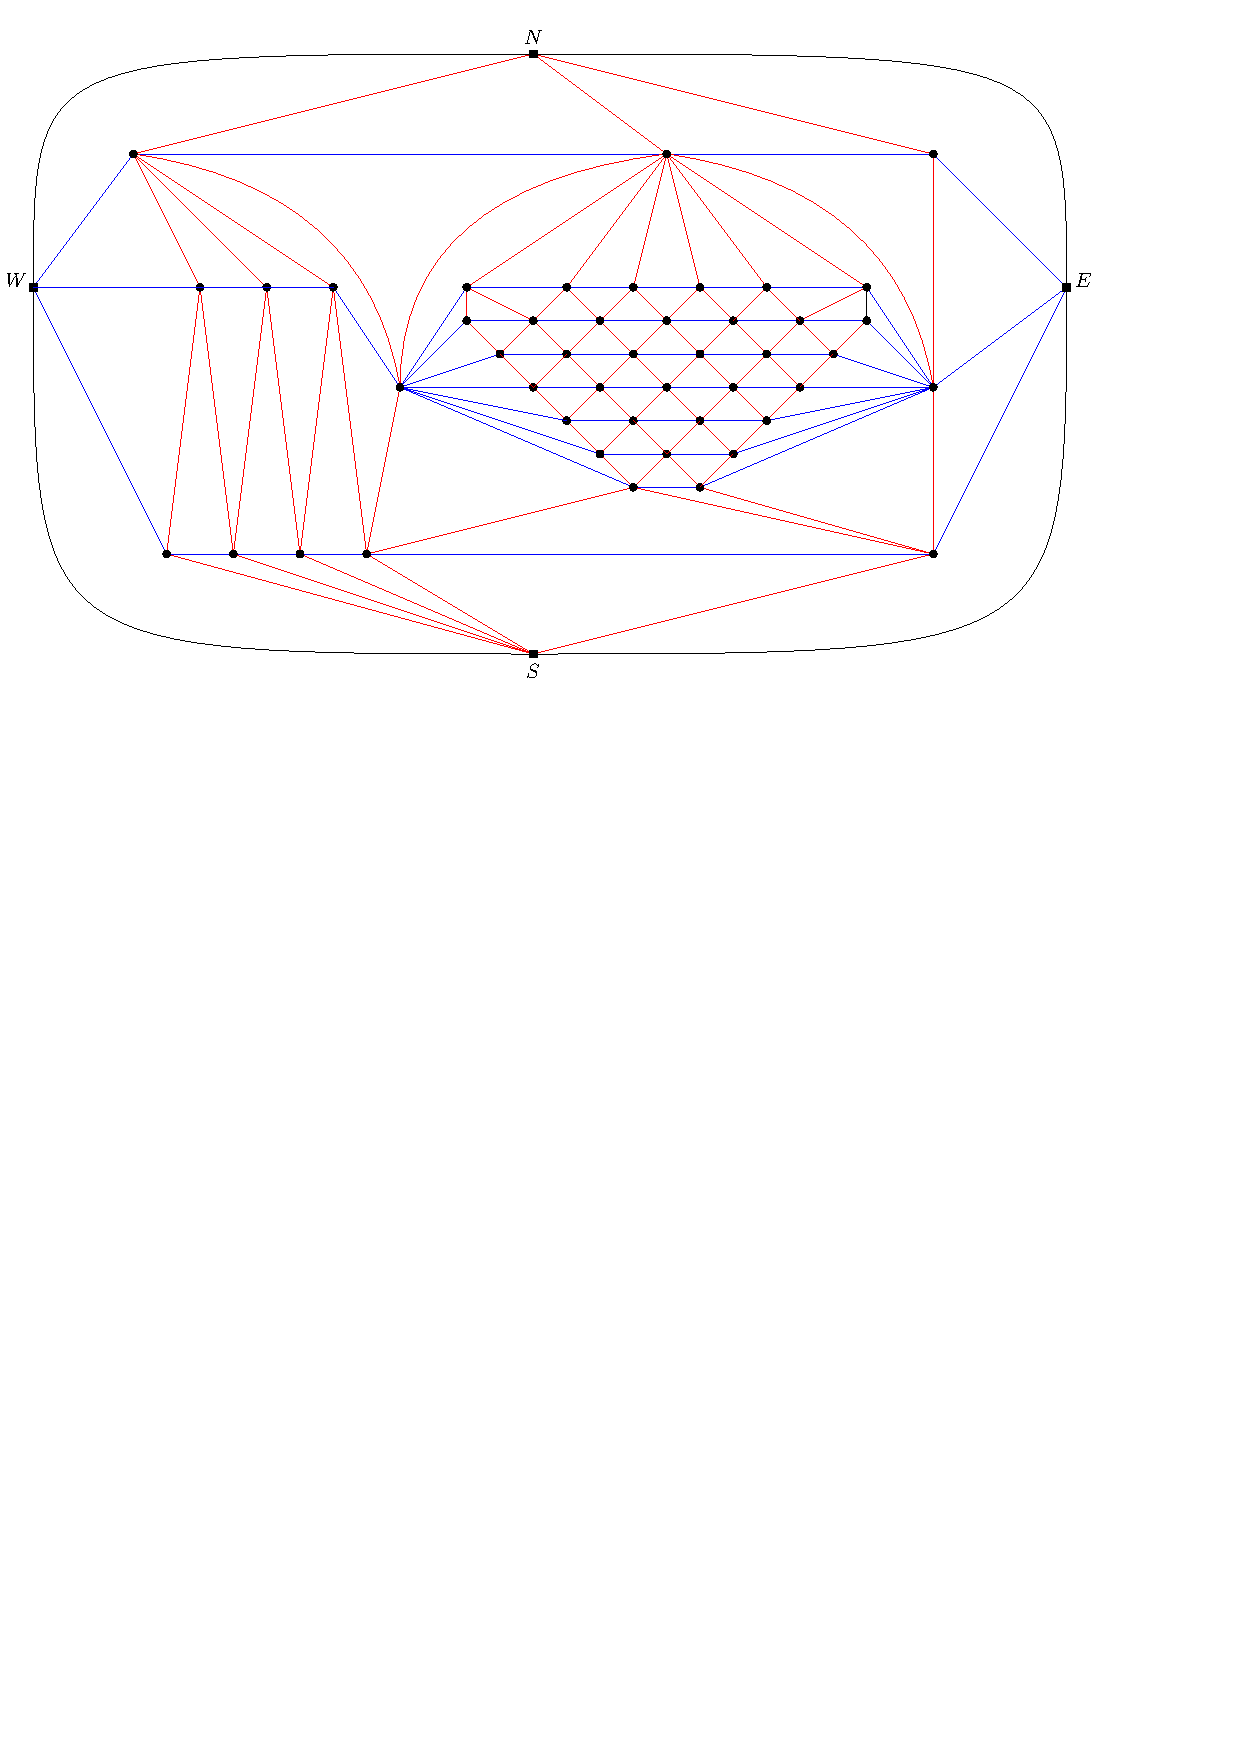
\includegraphics[width=\textwidth]{examples/img/vertWorstCase/sweepfinal}
      \caption{}
      \label{fig:ex:vert:sweepfinal}
    \end{subfigure}
    ~
    \begin{subfigure}[b]{.9 \textwidth}
      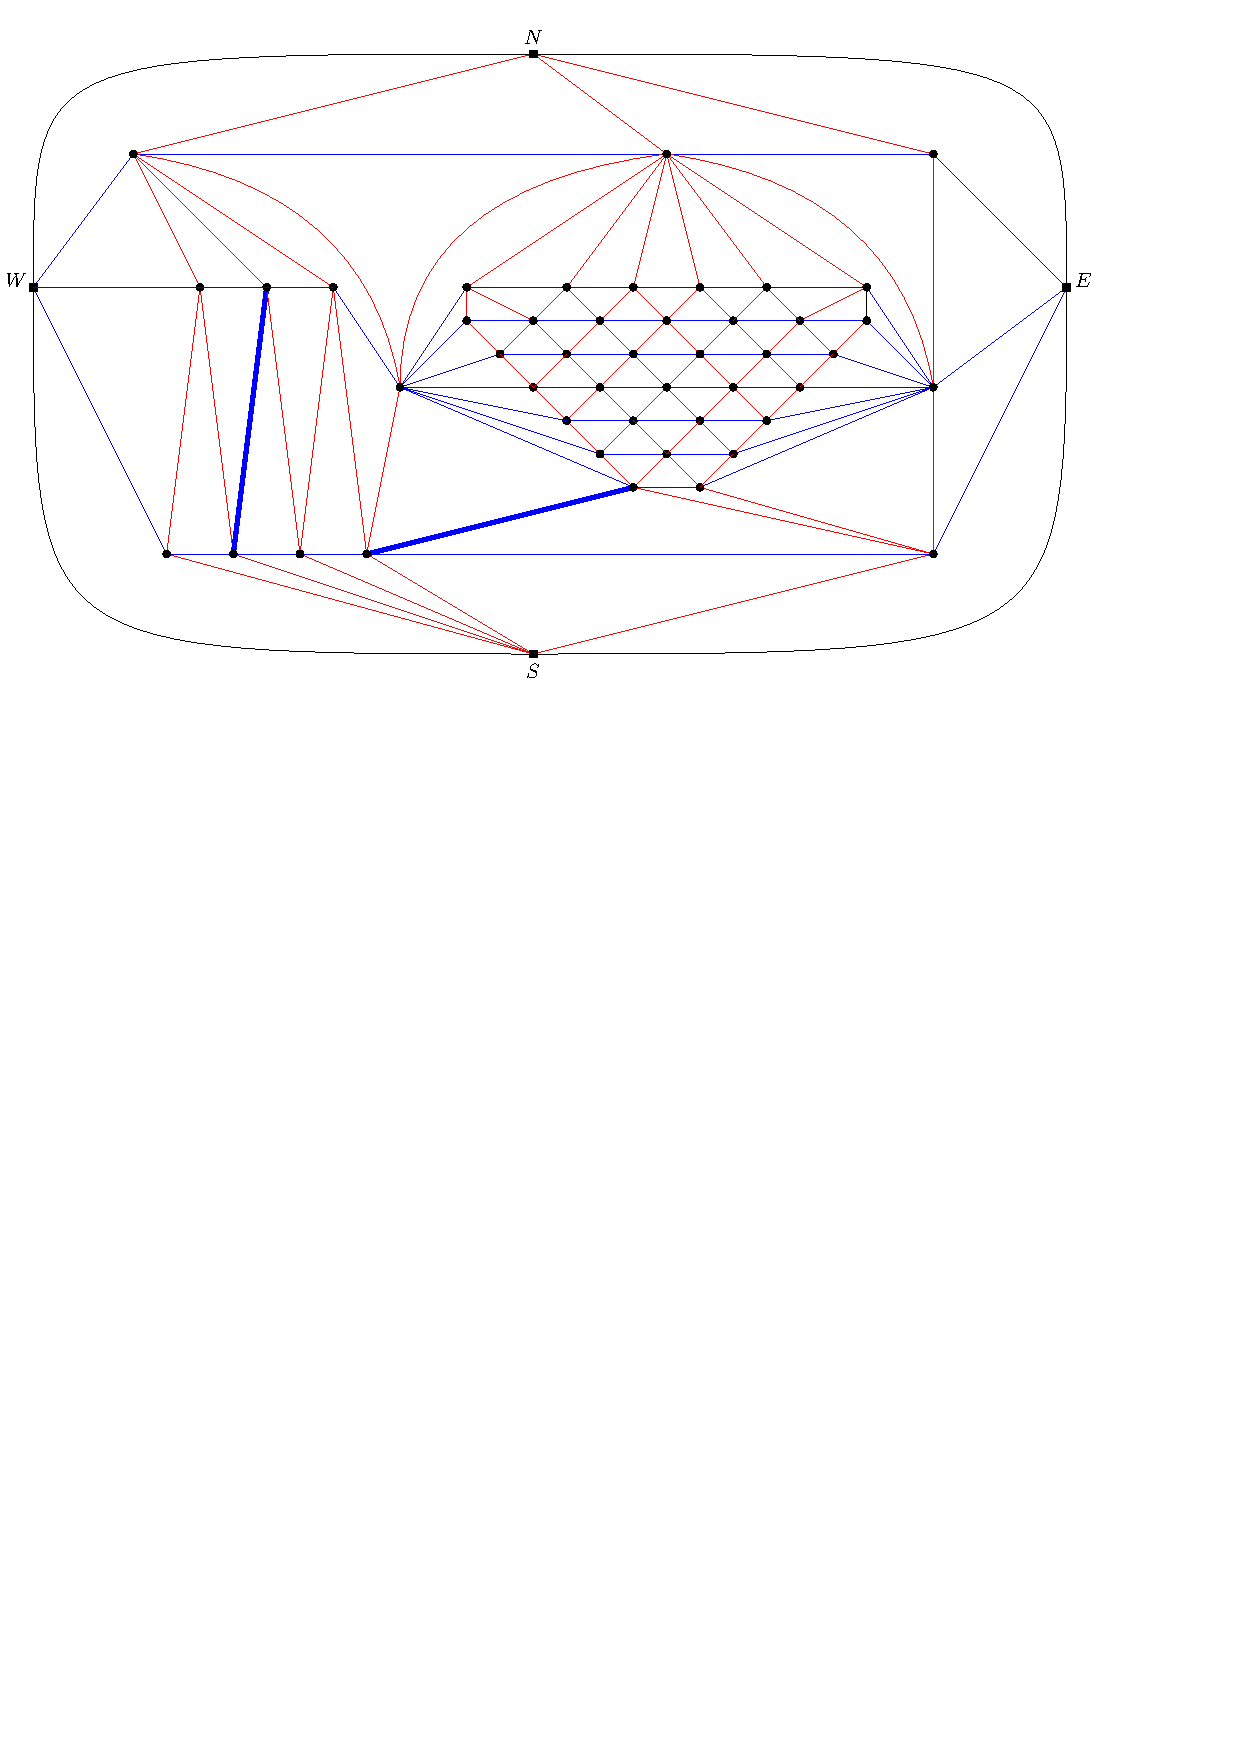
\includegraphics[width=\textwidth]{examples/img/vertWorstCase/subdiv1}
      \caption{}
      \label{fig:ex:vert:subdiv1}
    \end{subfigure}
  \caption{The steps of the algorithm}
  \label{}
\end{figure}



\begin{figure}
    \ContinuedFloat
    \begin{subfigure}[b]{.9 \textwidth}
      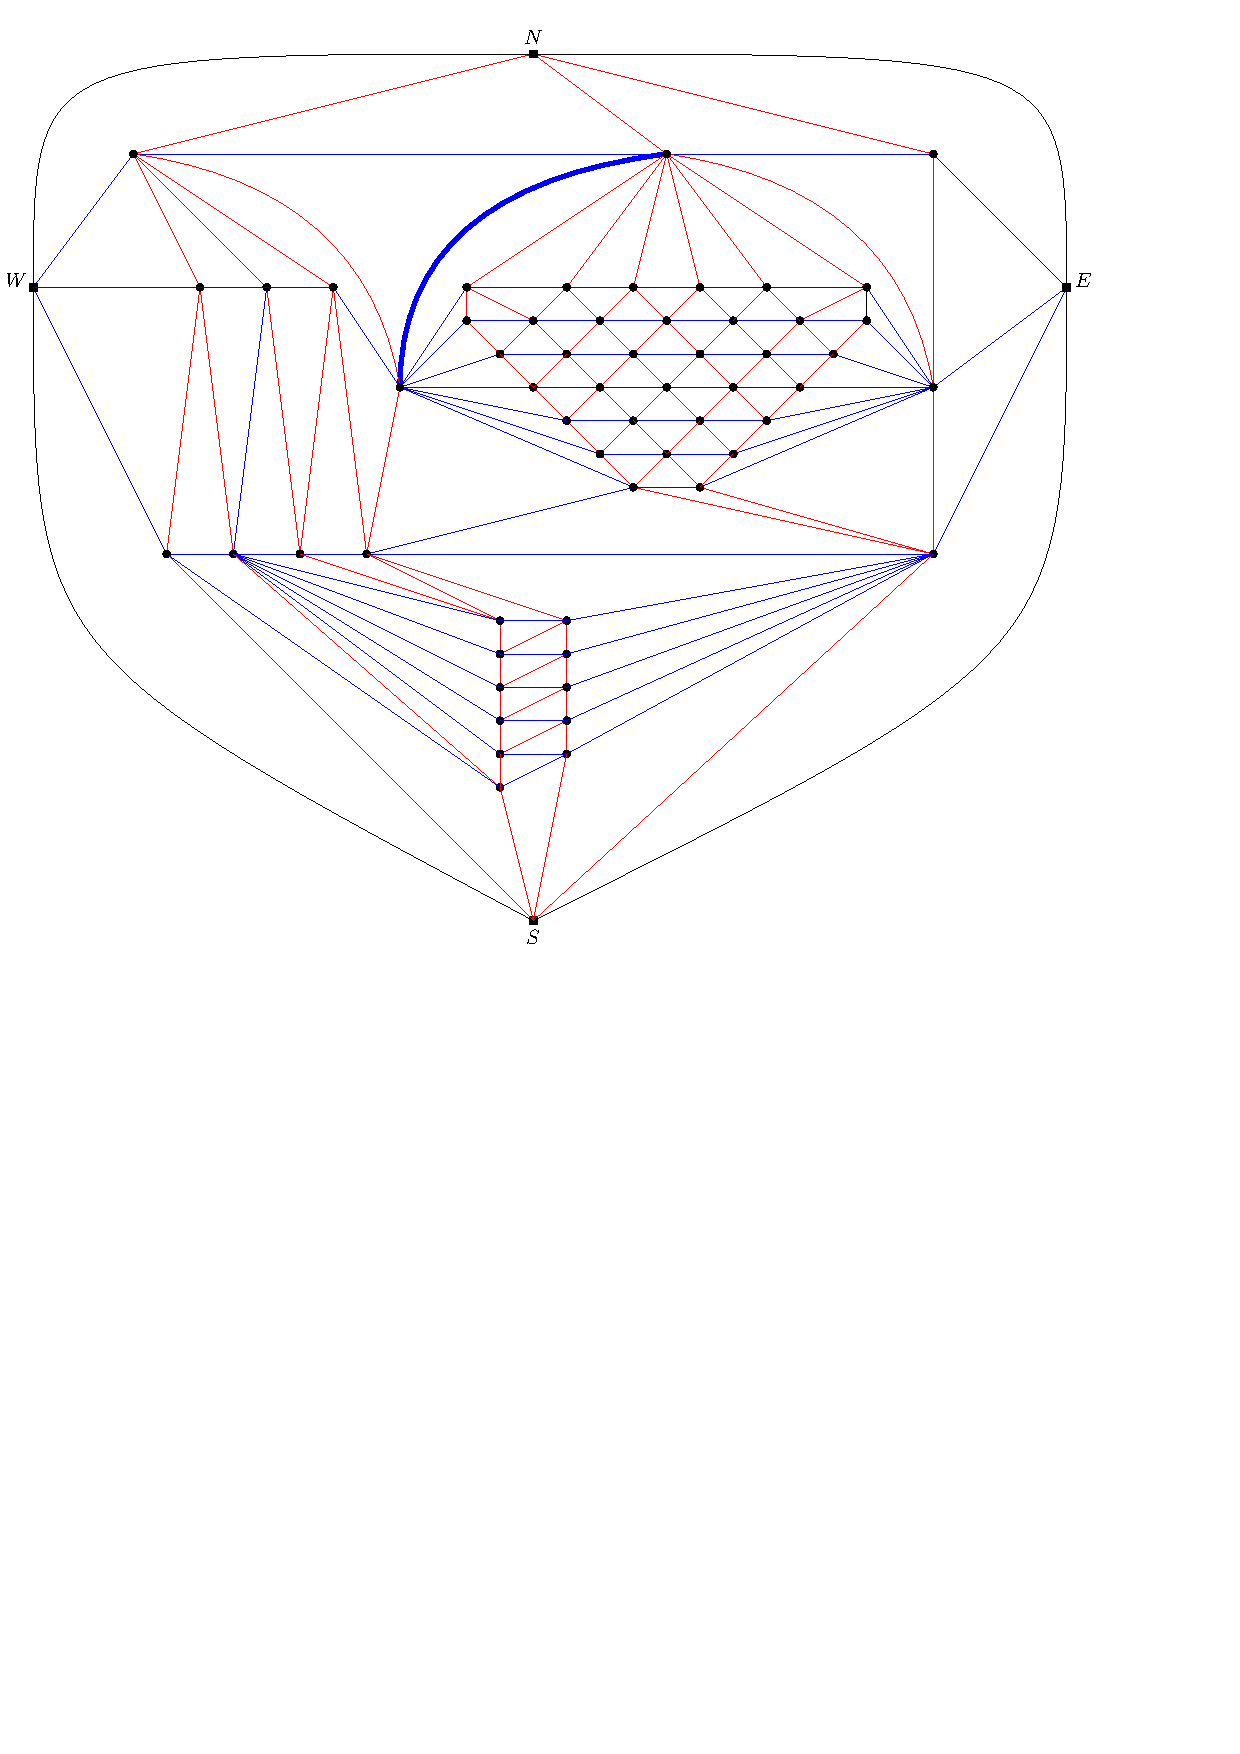
\includegraphics[width=\textwidth]{examples/img/vertWorstCase/subdivfinal}
      \caption{}
      \label{fig:ex:vert:subdivfinal}
    \end{subfigure}
  \caption{The steps of the algorithm}
  \label{}
\end{figure}
